\chapter{Umsetzung des Demonstrators}

\section{Beschreibung der Docker-basierten CI/CD-Pipeline}

\begin{figure}[h]
	\centering
	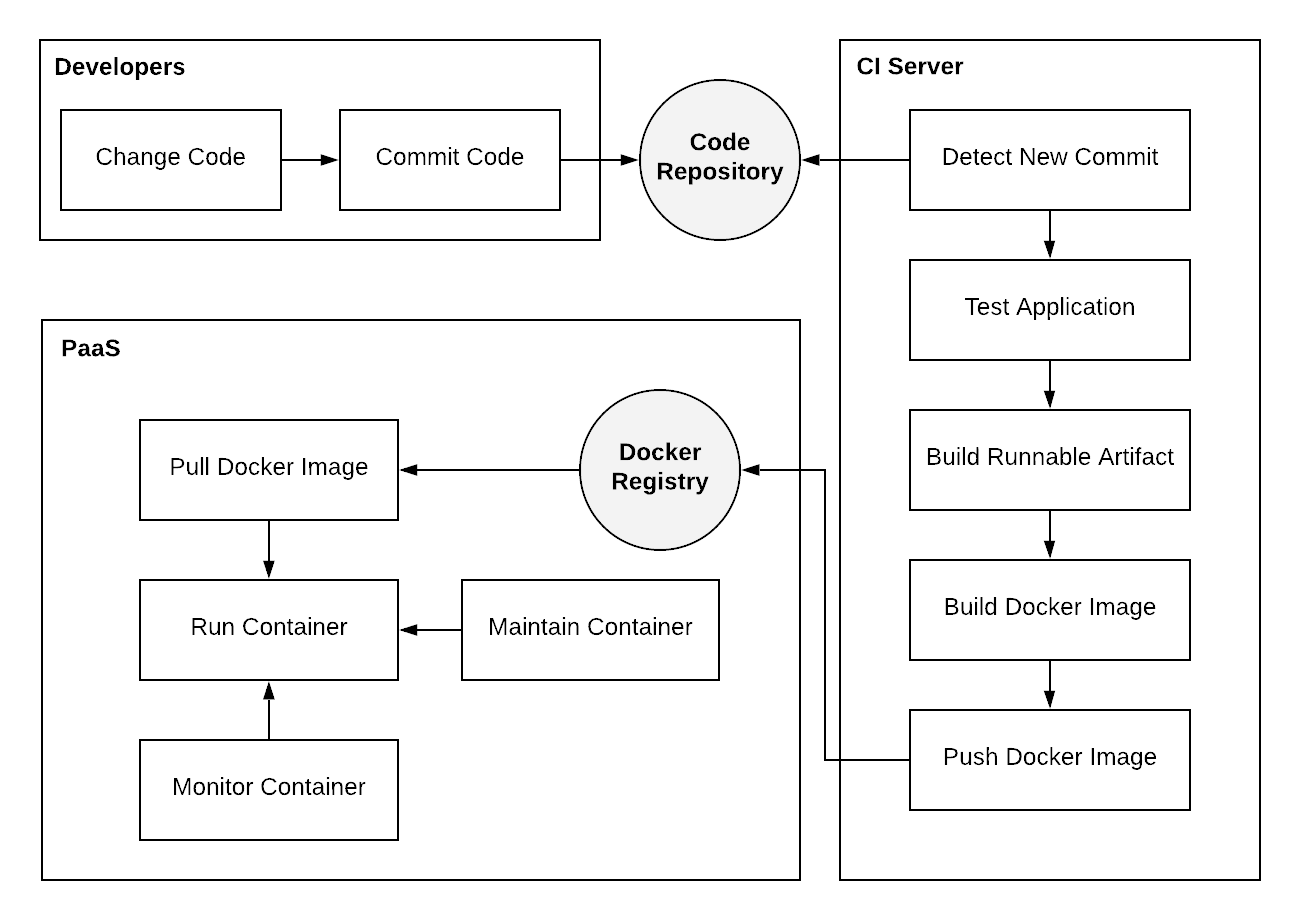
\includegraphics[width=\textwidth]{images/aktuelleInfrastruktur}
	\caption{Docker-basierte Infrastruktur bei C\&M}
	\label{fig:lokalesCluster}
\end{figure}

\begin{itemize}
	\item Abbildung zeigen
	\item Runner Server
	\item PaaS
	\item Ort der Docker Registry
	\item Ablauf eines Deployments beschreiben
\end{itemize}

\section{Beschreibung der Kubernetes-basierten CI/CD-Pipeline}

\section{Verteilung der TLM-Demo in einem lokalen Kubernetes-Cluster}

\begin{figure}[h]
	\centering
	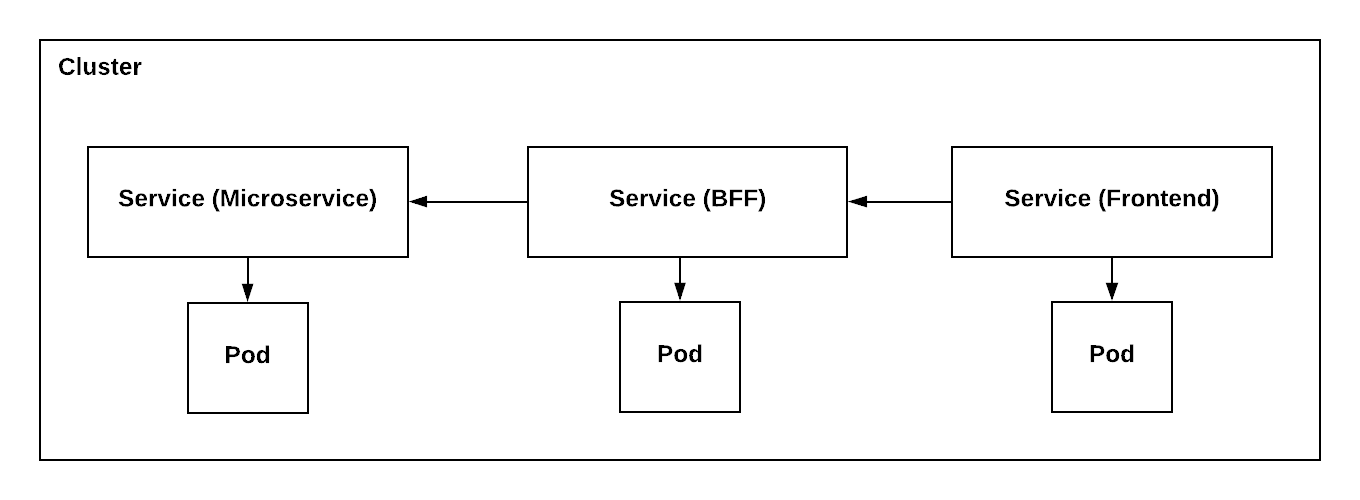
\includegraphics[width=\textwidth]{images/lokalesCluster}
	\caption{lokales Cluster}
	\label{fig:lokalesCluster}
\end{figure}

\subsection{Manuelle Verteilung}

\yamlcode{kubernetes/backend-pod.yaml}

\yamlcode{kubernetes/backend-service.yaml}

\yamlcode{kubernetes/bff-pod.yaml}

\yamlcode{kubernetes/bff-service.yaml}

\yamlcode{kubernetes/frontend-pod.yaml}

\yamlcode{kubernetes/frontend-service.yaml}

\begin{itemize}
	\item Minikube 
	\item Docker 
	\item Images bauen
	\item Cluster aufsetzen
	\item Pods (Konfiguration zeigen)
	\item Services (Konfiguration zeigen)
	\item Abbildung für Kommunikation
	\item Probleme
\end{itemize}

\subsection{Automatische Verteilung}

\section{Verteilung der TLM-Demo in einem realen Kubernetes-Cluster}